\section*{5.2 Phase estimation}

The Fourier transform is the key to a general procedure known as phase estimation, which in turn is the key for many quantum algorithms. Suppose a unitary operator $U$ has an eigenvector $|u\rangle$ with eigenvalue $e^{2 \pi i \varphi}$, where the value of $\varphi$ is unknown. The goal of the phase estimation algorithm is to estimate $\varphi$. To perform the estimation we assume that we have available black boxes (sometimes known as oracles) capable of preparing the state $|u\rangle$ and performing the controlled- $-U^{2^{j}}$ operation, for suitable non-negative integers $j$. The use of black boxes indicates that the phase estimation procedure is not a complete quantum algorithm in its own right. Rather, you should think of phase estimation as a kind of 'subroutine' or 'module' that, when combined with other subroutines, can be used to perform interesting computational tasks. In specific applications of the phase estimation procedure we shall do exactly this, describing how these black box operations are to be performed, and combining them with the phase estimation procedure to do genuinely useful tasks. For the moment, though, we will continue to imagine them as black boxes.

The quantum phase estimation procedure uses two registers. The first register contains $t$ qubits initially in the state $|0\rangle$. How we choose $t$ depends on two things: the number of digits of accuracy we wish to have in our estimate for $\varphi$, and with what probability we wish the phase estimation procedure to be successful. The dependence of $t$ on these quantities emerges naturally from the following analysis.

The second register begins in the state $|u\rangle$, and contains as many qubits as is necessary to store $|u\rangle$. Phase estimation is performed in two stages. First, we apply the circuit shown in Figure 5.2. The circuit begins by applying a Hadamard transform to the first register, followed by application of controlled- $U$ operations on the second register, with $U$ raised\\
to successive powers of two. The final state of the first register is easily seen to be:


\begin{align*}
\frac{1}{2^{t / 2}}\left(|0\rangle+e^{2 \pi i 2^{t-1} \varphi}|1\rangle\right)\left(|0\rangle+e^{2 \pi i 2^{t-2} \varphi}|1\rangle\right) & \ldots\left(|0\rangle+e^{2 \pi i 2^{0} \varphi}|1\rangle\right) \\
& =\frac{1}{2^{t / 2}} \sum_{k=0}^{2^{t}-1} e^{2 \pi i \varphi k}|k\rangle \tag{5.20}
\end{align*} 

We omit the second register from this description, since it stays in the state $|u\rangle$ throughout the computation.

\begin{figure}
\centering
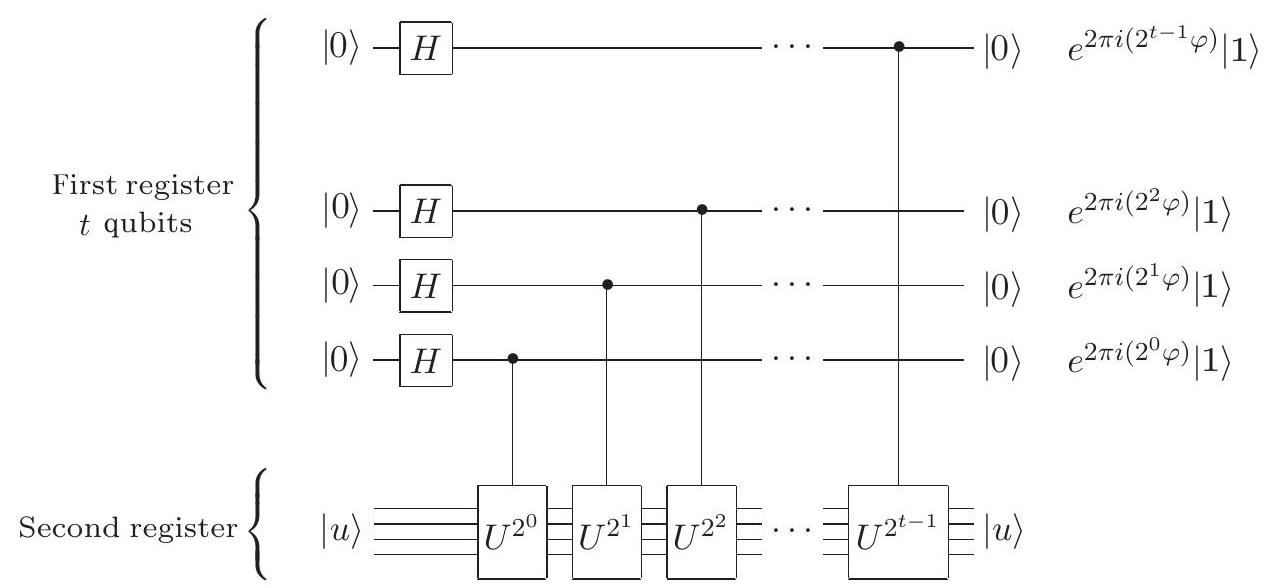
\includegraphics[width=0.75\linewidth]{Images/2024_05_17_6977ce60de6fd27aef98g-256}
\end{figure}

Figure 5.2. The first stage of the phase estimation procedure. Normalization factors of $1 / \sqrt{2}$ have been omitted, on the right.

Exercise 5.7: Additional insight into the circuit in Figure 5.2 may be obtained by showing, as you should now do, that the effect of the sequence of controlled- $U$ operations like that in Figure 5.2 is to take the state $|j\rangle|u\rangle$ to $|j\rangle U^{j}|u\rangle$. (Note that this does not depend on $|u\rangle$ being an eigenstate of $U$.)

The second stage of phase estimation is to apply the inverse quantum Fourier transform on the first register. This is obtained by reversing the circuit for the quantum Fourier transform in the previous section (Exercise 5.5), and can be done in $\Theta\left(t^{2}\right)$ steps. The third and final stage of phase estimation is to read out the state of the first register by doing a measurement in the computational basis. We will show that this provides a pretty good estimate of $\varphi$. An overall schematic of the algorithm is shown in Figure 5.3.

To sharpen our intuition as to why phase estimation works, suppose $\varphi$ may be expressed exactly in $t$ bits, as $\varphi=0 . \varphi_{1} \ldots \varphi_{t}$. Then the state (5.20) resulting from the first stage of phase estimation may be rewritten

\begin{equation*}
\frac{1}{2^{t / 2}}\left(|0\rangle+e^{2 \pi i 0 . \varphi_{t}}|1\rangle\right)\left(|0\rangle+e^{2 \pi i 0 . \varphi_{t-1} \varphi_{t}}|1\rangle\right) \ldots\left(|0\rangle+e^{2 \pi i 0 . \varphi_{1} \varphi_{2} \cdots \varphi_{t}}|1\rangle\right) \tag{5.21}
\end{equation*}

The second stage of phase estimation is to apply the inverse quantum Fourier transform. But comparing the previous equation with the product form for the Fourier transform, Equation (5.4), we see that the output state from the second stage is the product state $\left|\varphi_{1} \ldots \varphi_{t}\right\rangle$. A measurement in the computational basis therefore gives us $\varphi$ exactly!

\begin{figure}
\centering
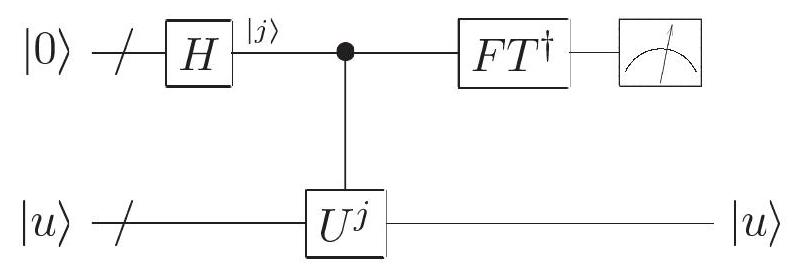
\includegraphics[width=0.75\linewidth]{Images/2024_05_17_6977ce60de6fd27aef98g-257}
\end{figure}

Figure 5.3. Schematic of the overall phase estimation procedure. The top $t$ qubits (the '/' denotes a bundle of wires, as usual) are the first register, and the bottom qubits are the second register, numbering as many as required to perform $U \cdot|u\rangle$ is an eigenstate of $U$ with eigenvalue $e^{2 \pi i \varphi}$. The output of the measurement is an approximation to $\varphi$ accurate to $t-\left\lceil\log \left(2+\frac{1}{2 \epsilon}\right)\right\rceil$ bits, with probability of success at least $1-\epsilon$.

Summarizing, the phase estimation algorithm allows one to estimate the phase $\varphi$ of an eigenvalue of a unitary operator $U$, given the corresponding eigenvector $|u\rangle$. An essential feature at the heart of this procedure is the ability of the inverse Fourier transform to perform the transformation

\begin{equation*}
\frac{1}{2^{t / 2}} \sum_{j=0}^{2^{t}-1} e^{2 \pi i \varphi j}|j\rangle|u\rangle \rightarrow|\tilde{\varphi}\rangle|u\rangle \tag{5.22}
\end{equation*}

where $|\tilde{\varphi}\rangle$ denotes a state which is a good estimator for $\varphi$ when measured.

\subsection*{5.2.1 Performance and requirements}

The above analysis applies to the ideal case, where $\varphi$ can be written exactly with a $t$ bit binary expansion. What happens when this is not the case? It turns out that the procedure we have described will produce a pretty good approximation to $\varphi$ with high probability, as foreshadowed by the notation used in (5.22). Showing this requires some careful manipulations.

Let $b$ be the integer in the range 0 to $2^{t}-1$ such that $b / 2^{t}=0 . b_{1} \ldots b_{t}$ is the best $t$ bit approximation to $\varphi$ which is less than $\varphi$. That is, the difference $\delta \equiv \varphi-b / 2^{t}$ between $\varphi$ and $b / 2^{t}$ satisfies $0 \leq \delta \leq 2^{-t}$. We aim to show that the observation at the end of the phase estimation procedure produces a result which is close to $b$, and thus enables us to estimate $\varphi$ accurately, with high probability. Applying the inverse quantum Fourier transform to the state (5.20) produces the state

\begin{equation*}
\frac{1}{2^{t}} \sum_{k, l=0}^{2^{t}-1} e^{\frac{-2 \pi i k l}{2^{t}}} e^{2 \pi i \varphi k}|l\rangle \tag{5.23}
\end{equation*}

Let $\alpha_{l}$ be the amplitude of $\left|(b+l)\left(\bmod 2^{t}\right)\right\rangle$,

\begin{equation*}
\alpha_{l} \equiv \frac{1}{2^{t}} \sum_{k=0}^{2^{t}-1}\left(e^{2 \pi i\left(\varphi-(b+l) / 2^{t}\right)}\right)^{k} \tag{5.24}
\end{equation*}

This is the sum of a geometric series, so

\begin{equation*}
\alpha_{l}=\frac{1}{2^{t}}\left(\frac{1-e^{2 \pi i\left(2^{t} \varphi-(b+l)\right)}}{1-e^{2 \pi i\left(\varphi-(b+l) / 2^{t}\right)}}\right) \tag{5.25}
\end{equation*}

\begin{equation*}
=\frac{1}{2^{t}}\left(\frac{1-e^{2 \pi i\left(2^{t} \delta-l\right)}}{1-e^{2 \pi i\left(\delta-l / 2^{t}\right)}}\right) \tag{5.26}
\end{equation*}

Suppose the outcome of the final measurement is $m$. We aim to bound the probability of obtaining a value of $m$ such that $|m-b|>e$, where $e$ is a positive integer characterizing our desired tolerance to error. The probability of observing such an $m$ is given by

\begin{equation*}
p(|m-b|>e)=\sum_{-2^{t-1}<l \leq-(e+1)}\left|\alpha_{l}\right|^{2}+\sum_{e+1 \leq l \leq 2^{t-1}}\left|\alpha_{l}\right|^{2} \tag{5.27}
\end{equation*}

But for any real $\theta,|1-\exp (i \theta)| \leq 2$, so

\begin{equation*}
\left|\alpha_{l}\right| \leq \frac{2}{2^{t} \mid 1-e^{2 \pi i\left(\delta-l / 2^{t}\right) \mid}} \tag{5.28}
\end{equation*}

By elementary geometry or calculus $|1-\exp (i \theta)| \geq 2|\theta| / \pi$ whenever $-\pi \leq \theta \leq \pi$. But when $-2^{t-1}<l \leq 2^{t-1}$ we have $-\pi \leq 2 \pi\left(\delta-l / 2^{t}\right) \leq \pi$. Thus

\begin{equation*}
\left|\alpha_{l}\right| \leq \frac{1}{2^{t+1}\left(\delta-l / 2^{t}\right)} \tag{5.29}
\end{equation*}

Combining (5.27) and (5.29) gives

\begin{equation*}
p(|m-b|>e) \leq \frac{1}{4}\left[\sum_{l=-2^{t-1}+1}^{-(e+1)} \frac{1}{\left(l-2^{t} \delta\right)^{2}}+\sum_{l=e+1}^{2^{t-1}} \frac{1}{\left(l-2^{t} \delta\right)^{2}}\right] \tag{5.30}
\end{equation*}

Recalling that $0 \leq 2^{t} \delta \leq 1$, we obtain


\begin{align*}
p(|m-b|>e) & \leq \frac{1}{4}\left[\sum_{l=-2^{t-1+1}}^{-(e+1)} \frac{1}{l^{2}}+\sum_{l=e+1}^{2^{t-1}} \frac{1}{(l-1)^{2}}\right]  \tag{5.31}\\
& \leq \frac{1}{2} \sum_{l=e}^{2^{t-1}-1} \frac{1}{l^{2}}  \tag{5.32}\\
& \leq \frac{1}{2} \int_{e-1}^{2^{t-1}-1} d l \frac{1}{l^{2}}  \tag{5.33}\\
& =\frac{1}{2(e-1)} \tag{5.34}
\end{align*} 

Suppose we wish to approximate $\varphi$ to an accuracy $2^{-n}$, that is, we choose $e=2^{t-n}-1$. By making use of $t=n+p$ qubits in the phase estimation algorithm we see from (5.34) that the probability of obtaining an approximation correct to this accuracy is at least $1-1 / 2\left(2^{p}-2\right)$. Thus to successfully obtain $\varphi$ accurate to $n$ bits with probability of success at least $1-\epsilon$ we choose

\begin{equation*}
t=n+\left\lceil\log \left(2+\frac{1}{2 \epsilon}\right)\right\rceil \tag{5.35}
\end{equation*}

In order to make use of the phase estimation algorithm, we need to be able to prepare an eigenstate $|u\rangle$ of $U$. What if we do not know how to prepare such an eigenstate? Suppose that we prepare some other state $|\psi\rangle$ in place of $|u\rangle$. Expanding this state in terms of eigenstates $|u\rangle$ of $U$ gives $|\psi\rangle=\sum_{u} c_{u}|u\rangle$. Suppose the eigenstate $|u\rangle$ has eigenvalue $e^{2 \pi i \varphi_{u}}$. Intuitively, the result of running the phase estimation algorithm will be to give\\
as output a state close to $\sum_{u} c_{u}\left|\widetilde{\varphi_{u}}\right\rangle|u\rangle$, where $\widetilde{\varphi_{u}}$ is a pretty good approximation to the phase $\varphi_{u}$. Therefore, we expect that reading out the first register will give us a good approximation to $\varphi_{u}$, where $u$ is chosen at random with probability $\left|c_{u}\right|^{2}$. Making this argument rigorous is left for Exercise 5.8. This procedure allows us to avoid preparing a (possibly unknown) eigenstate, at the cost of introducing some additional randomness into the algorithm.

Exercise 5.8: Suppose the phase estimation algorithm takes the state $|0\rangle|u\rangle$ to the state $\left|\widetilde{\varphi_{u}}\right\rangle|u\rangle$, so that given the input $|0\rangle\left(\sum_{u} c_{u}|u\rangle\right)$, the algorithm outputs $\sum_{u} c_{u}\left|\widetilde{\varphi_{u}}\right\rangle|u\rangle$. Show that if $t$ is chosen according to (5.35), then the probability for measuring $\varphi_{u}$ accurate to $n$ bits at the conclusion of the phase estimation algorithm is at least $\left|c_{u}\right|^{2}(1-\epsilon)$.

Why is phase estimation interesting? For its own sake, phase estimation solves a problem which is both non-trivial and interesting from a physical point of view: how to estimate the eigenvalue associated to a given eigenvector of a unitary operator. Its real use, though, comes from the observation that other interesting problems can be reduced to phase estimation, as will be shown in subsequent sections. The phase estimation algorithm is summarized below.

\textbf{Algorithm: Quantum phase estimation}

Inputs: (1) A black box wich performs a controlled- $U^{j}$ operation, for integer $j$, (2) an eigenstate $|u\rangle$ of $U$ with eigenvalue $e^{2 \pi i \varphi_{u}}$, and (3) $t=n+\left\lceil\log \left(2+\frac{1}{2 \epsilon}\right)\right\rceil$ qubits initialized to $|0\rangle$.

Outputs: An $n$-bit approximation $\widetilde{\varphi_{u}}$ to $\varphi_{u}$.

Runtime: $O\left(t^{2}\right)$ operations and one call to controlled- $U^{j}$ black box. Succeeds with probability at least $1-\epsilon$.

\textbf{Procedure:}
\begin{enumerate}
  \item $\quad|0\rangle|u\rangle$
\end{enumerate}

initial state\\
2. $\quad \rightarrow \frac{1}{\sqrt{2^{t}}} \sum_{j=0}^{2^{t}-1}|j\rangle|u\rangle$

create superposition\\
3. $\left.\quad \rightarrow \frac{1}{\sqrt{2^{t}}} \sum_{j=0}^{2^{t}-1}|j\rangle U^{j} \right\rvert\, u$

apply black box

$=\frac{1}{\sqrt{2^{t}}} \sum_{j=0}^{2^{t}-1} e^{2 \pi i j \varphi_{u}}|j\rangle|u\rangle$

result of black box\\
4. $\quad \rightarrow\left|\widetilde{\varphi_{u}}\right\rangle|u\rangle$

apply inverse Fourier transform\\
5. $\quad \rightarrow \widetilde{\varphi_{u}}$

measure first register

Exercise 5.9: Let $U$ be a unitary transform with eigenvalues $\pm 1$, which acts on a state $|\psi\rangle$. Using the phase estimation procedure, construct a quantum circuit to collapse $|\psi\rangle$ into one or the other of the two eigenspaces of $U$, giving also a\\
classical indicator as to which space the final state is in. Compare your result with Exercise 4.34.